\documentclass{standalone}
\usepackage{tikz}
\usetikzlibrary{calc}
\begin{document}

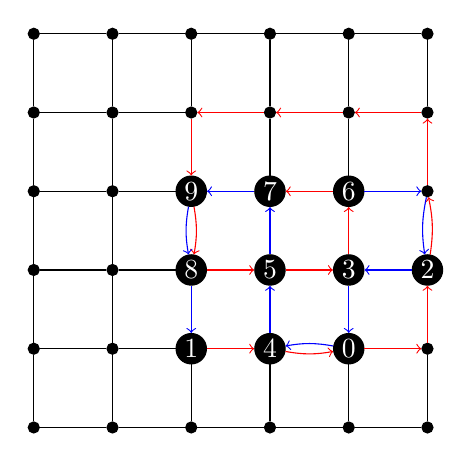
\begin{tikzpicture}[
  every node/.style={circle, inner sep=1pt, minimum size=4pt, draw, fill=black}
]
  \node (a) at (0,0) {};
  \node (b) at (1,0) {};
  \node (c) at (2,0) {};
  \node (d) at (3,0) {};
  \node (e) at (4,0) {};
  \node (f) at (5,0) {};
  
  \node (a1) at (0,1) {};
  \node (b1) at (1,1) {};
  \node (c1) at (2,1) {\textcolor{white}{1}};
  \node (d1) at (3,1) {\textcolor{white}{4}};
  \node (e1) at (4,1) {\textcolor{white}{0}};
  \node (f1) at (5,1) {};

  \node (a2) at (0,2) {};
  \node (b2) at (1,2) {};
  \node (c2) at (2,2) {\textcolor{white}{8}};
  \node (d2) at (3,2) {\textcolor{white}{5}};
  \node (e2) at (4,2) {\textcolor{white}{3}};
  \node (f2) at (5,2) {\textcolor{white}{2}};

  \node (a3) at (0,3) {};
  \node (b3) at (1,3) {};
  \node (c3) at (2,3) {\textcolor{white}{9}};
  \node (d3) at (3,3) {\textcolor{white}{7}};
  \node (e3) at (4,3) {\textcolor{white}{6}};
  \node (f3) at (5,3) {};

  \node (a4) at (0,4) {};
  \node (b4) at (1,4) {};
  \node (c4) at (2,4) {};
  \node (d4) at (3,4) {};
  \node (e4) at (4,4) {};
  \node (f4) at (5,4) {};

  \node (a5) at (0,5) {};
  \node (b5) at (1,5) {};
  \node (c5) at (2,5) {};
  \node (d5) at (3,5) {};
  \node (e5) at (4,5) {};
  \node (f5) at (5,5) {};


  \draw (a) edge[-](b);
  \draw (b) edge[-](c);
  \draw (c) edge[-](d);
  \draw (d) edge[-](e);
  \draw (e) edge[-](f);

  \draw (a) edge[-](a1);
  \draw (b) edge[-](b1);
  \draw (c) edge[-](c1);
  \draw (d) edge[-](d1);
  \draw (e) edge[-](e1);
  \draw (f) edge[-](f1);


  \draw (a1) edge[-](b1);
  \draw (b1) edge[-](c1);
  \draw (c1) edge[->,red](d1);
  \draw[->, red] (d1) to[bend right=10] (e1);
  \draw[<-, blue] (d1) to[bend left=10] (e1);
  \draw (e1) edge[->,red](f1);

  \draw (a1) edge[-](a2);
  \draw (b1) edge[-](b2);
  \draw (c1) edge[<-,blue](c2);
  \draw (d1) edge[->,blue](d2);
  \draw (e1) edge[<-,blue](e2);
  \draw (f1) edge[->,red](f2);


  \draw (a2) edge[-](b2);
  \draw (b2) edge[-](c2);
  \draw (c2) edge[->,red](d2);
  \draw (d2) edge[->,red](e2);
  \draw (e2) edge[<-,blue](f2);

  \draw (a2) edge[-](a3);
  \draw (b2) edge[-](b3);
  \draw[<-, red] (c2) to[bend right=10] (c3);
  \draw[<-, blue] (c2) to[bend left=10] (c3);
  \draw (d2) edge[->,blue](d3);
  \draw (e2) edge[->,red](e3);
  \draw[->, red] (f2) to[bend right=10] (f3);
  \draw[<-, blue] (f2) to[bend left=10] (f3);


  \draw (a3) edge[-](b3);
  \draw (b3) edge[-](c3);
  \draw (c3) edge[<-,blue](d3);
  \draw (d3) edge[<-,red](e3);
  \draw (e3) edge[->,blue](f3);

  \draw (a3) edge[-](a4);
  \draw (b3) edge[-](b4);
  \draw (c3) edge[<-,red](c4);
  \draw (d3) edge[-](d4);
  \draw (e3) edge[-](e4);
  \draw (f3) edge[->,red](f4);


  \draw (a4) edge[-](b4);
  \draw (b4) edge[-](c4);
  \draw (c4) edge[<-,red](d4);
  \draw (d4) edge[<-,red](e4);
  \draw (e4) edge[<-,red](f4);

  \draw (a4) edge[-](a5);
  \draw (b4) edge[-](b5);
  \draw (c4) edge[-](c5);
  \draw (d4) edge[-](d5);
  \draw (e4) edge[-](e5);
  \draw (f4) edge[-](f5);


  \draw (a5) edge[-](b5);
  \draw (b5) edge[-](c5);
  \draw (c5) edge[-](d5);
  \draw (d5) edge[-](e5);
  \draw (e5) edge[-](f5);
\end{tikzpicture}

\end{document}
Pfad 1:
[2, 5, 1, 3, 10, 9, 6, 4, 7, 8]
Pfad 2:
[7, 3, 4, 1, 5, 6, 8, 10, 9, 2]
\draw[<-, red] (c2) to[bend right=10] (c3);
  \draw[<-, blue] (c2) to[bend left=10] (c3);
\node (a) at (0,3) {\textcolor{white}{1}};
\node (b) at (1,3) {};